\paragraph{Sơ đồ tuần tự luồng nghe thử mẫu giọng nói của nhân vật}

Luồng nghiệp vụ này mô tả
quá trình Khách vãng lai (Guest)
thực hiện click nghe thử giọng nói của nhân vật.
Dữ liệu âm thanh được phát trực tiếp trên Web Frontend
từ public URL lưu trong thông tin nhân vật.

\begin{figure}[H]
\centering
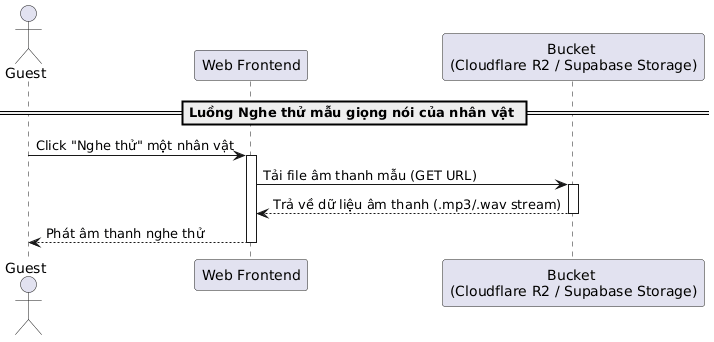
\includegraphics[scale = 0.5]{contents/Sequence/UML-Sequence-GuestPersonaVoicePreview.png}
\caption{Sơ đồ tuần tự luồng nghe thử mẫu giọng nói}
\end{figure}

\subparagraph{Các thành phần tham gia}

\begin{table}[H]
\centering
\renewcommand{\arraystretch}{1.3}

\begin{tabular}{|l|l|p{5cm}|}
\hline
\textbf{Thành phần} & \textbf{Phân loại} & \textbf{Vai trò trong hệ thống} \\ \hline
Guest & Actor & Khách vãng lai tương tác nghe thử. \\ \hline
Web Frontend & Component & Giao diện web Next.js. \\ \hline %%%% Component & Nhận và phát luồng âm thanh nghe thử. \\ \hline
Storage Bucket & Storage & Lưu trữ và cung cấp tệp tin âm thanh của nhân vật thông qua URL công khai. \\ \hline
\end{tabular}
\caption{Các thành phần tham gia luồng nghe thử mẫu giọng nói}
\end{table}

\subparagraph{Mô tả tổng quan}

\begin{itemize}

\item \textbf{Yêu cầu nghe thử:}
Khách vãng lai chọn chức năng nghe thử giọng nói
của một nhân vật trên trang chủ.

\item \textbf{Tải luồng âm thanh:}
Giao diện gửi yêu cầu tải luồng âm thanh trực tiếp
đến địa chỉ kho chứa tệp công khai của nhân vật mà không cần qua cổng API.

\item \textbf{Nhận âm thanh:}
Kho chứa trả về dữ liệu luồng âm thanh của nhân vật dưới dạng tệp âm thanh.

\item \textbf{Phát âm thanh:}
Giao diện tiếp nhận luồng dữ liệu
và phát âm thanh trực tiếp cho người dùng nghe.
\end{itemize}
